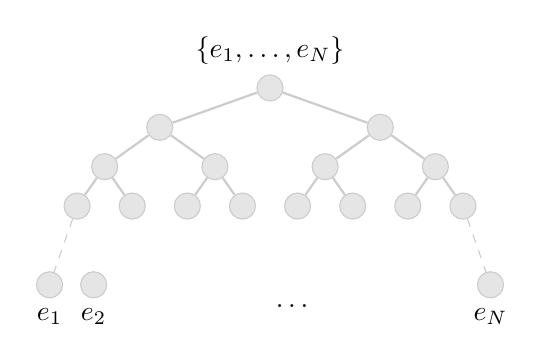
\begin{tikzpicture}
[   cnode/.style={draw=gray!40,fill=gray!20,minimum width=0.2mm,circle},
    cline/.style={gray!40,thick}
]

\def\stepx{0.7};
\def\stepy{0.5};

\node[cnode] (000) at (-0.5*\stepx,-2*\stepy) {};
\node[cnode] (001) at (-1.5*\stepx,-2*\stepy) {};
\node[cnode] (010) at (-2.5*\stepx,-2*\stepy) {};
\node[cnode] (011) at (-3.5*\stepx,-2*\stepy) {};
\node[cnode] (100) at (0.5*\stepx,-2*\stepy) {};
\node[cnode] (101) at (1.5*\stepx,-2*\stepy) {};
\node[cnode] (110) at (2.5*\stepx,-2*\stepy) {};
\node[cnode] (111) at (3.5*\stepx,-2*\stepy) {};

\node[cnode] (00) at (-3*\stepx,-\stepy) {};
\node[cnode] (01) at (-1*\stepx,-\stepy) {};
\node[cnode] (10) at (1*\stepx,-\stepy) {};
\node[cnode] (11) at (3*\stepx,-\stepy) {};

\node[cnode] (0) at (-2*\stepx,0*\stepy) {};
\node[cnode] (1) at (2*\stepx,0*\stepy) {};

\node[cnode, label=90:{$\{e_1, \ldots, e_N\}$}] (root) at (0,\stepy) {};

\node[cnode, label=270:{$e_1$}] (t1) at (-4*\stepx,-4*\stepy) {};
\node[cnode, label=270:{$e_2$}] (t2) at (-3.2*\stepx,-4*\stepy) {};
\node[label=270:{$\ldots$}] at (0.4*\stepx, -4*\stepy) {};
\node[cnode, label=270:{$e_N$}] (tn) at (4*\stepx,-4*\stepy) {};

\draw[cline] (root) -- (0) {};
\draw[cline] (root) -- (1) {};

\draw[cline] (00) -- (0) {};
\draw[cline] (10) -- (1) {};
\draw[cline] (01) -- (0) {};
\draw[cline] (11) -- (1) {};

\draw[cline] (01) -- (000) {};
\draw[cline] (01) -- (001) {};
\draw[cline] (00) -- (010) {};
\draw[cline] (00) -- (011) {};
\draw[cline] (10) -- (100) {};
\draw[cline] (10) -- (101) {};
\draw[cline] (11) -- (110) {};
\draw[cline] (11) -- (111) {};

\draw[dashed,gray!40] (011) -- (t1) {};
\draw[dashed,gray!40] (111) -- (tn) {};

\end{tikzpicture}